\documentclass[11pt]{article}
\usepackage[margin=1in]{geometry}
\usepackage[T1]{fontenc}
\usepackage[utf8]{inputenc}
\usepackage{graphicx}
\usepackage{booktabs}
\usepackage{caption}
\usepackage{hyperref}
\usepackage{array}
\usepackage{float}
\usepackage{enumitem}
\usepackage{amsmath}
\usepackage{amssymb}
\usepackage{tabularx}
\usepackage{longtable}
\usepackage{xcolor}

\graphicspath{{assets/}}
\hypersetup{
  colorlinks=true,
  linkcolor=blue,
  urlcolor=blue,
  citecolor=blue,
  pdfauthor={junior yu},
  pdftitle={Benchmark-Style Cross-Dataset Cell Type Annotation with scGPT on Human Gut Atlas Transfer},
}

\title{Benchmark-Style Cross-Dataset Cell Type Annotation with scGPT on Human Gut Atlas Transfer}
\author{junior yu}
\date{\today}

\begin{document}
\maketitle

\begin{abstract}
We study cross-dataset cell type annotation under domain shift using scGPT on the human gut atlas.
The task pairs a reference atlas of 14{,}159 cells with a 11{,}982-cell query atlas; after harmonization, 9 labels and 128 shared genes remain.
We train a compact scGPT transformer for five epochs with checkpoint-resume support and evaluate query accuracy, balanced accuracy, macro-F1, ARI, and NMI.
Final query performance is 18.96\% accuracy, 16.64\% balanced accuracy, 11.65\% macro-F1, 3.47\% ARI, and 5.39\% NMI.
Although the current model is not yet a strong benchmark contender, the experiment establishes a reproducible end-to-end transfer pipeline with complete artifacts and a baseline reporting structure.
\end{abstract}

\section{Introduction}
Cross-dataset cell type annotation is a stringent test of representation learning in single-cell transcriptomics because the model must transfer labels across batches, donors, and experiments.
This benchmark is more informative than a random within-dataset split because it measures whether the learned representation remains useful after a genuine domain shift.

In this manuscript we convert an initial smoke test into a benchmark-style transfer study on the human gut atlas.
Our objective is not to claim state-of-the-art accuracy, but to establish a reproducible protocol: a fixed task definition, deterministic preprocessing, recoverable training, standard metrics, and exportable analysis artifacts.

The main contribution is operational rather than algorithmic.
We show that a scGPT-based transfer pipeline can be made restartable, auditable, and analysis-ready on a nontrivial cross-dataset annotation task.
That matters because the failure mode of many pilot runs is not weak performance alone, but a workflow that cannot be repeated, resumed, or inspected.
Here the pipeline now survives those issues.

\section{Related Work}
Representation learning for single-cell transcriptomics has moved from feature engineering toward transformer-based foundation models.
scGPT introduced a generative transformer backbone for single-cell data and established a template for learning shared latent structure from large atlases.
In parallel, automated annotation systems such as CellTypist demonstrated that label transfer can be made accurate and practical when a stable reference atlas is available.
Our work sits between these two lines: we use scGPT as the backbone, but evaluate it in a CellTypist-like cross-atlas transfer setting where the key question is annotation robustness under domain shift.

The paper-style benchmark framing is also deliberate.
Instead of treating the result as a one-off fine-tuning run, we define a repeatable benchmark target with explicit artifacts, common metrics, and a baseline suite.
That makes the output suitable for incremental research: the same protocol can absorb more seeds, stronger models, different gene-selection strategies, or additional transfer datasets without changing the reporting structure.

\section{Methods}
\subsection{Task definition}
We consider a paired reference/query label-transfer problem on the human gut atlas.
The model is trained on the reference atlas and evaluated on the query atlas after label harmonization.
Because the protocol is cross-dataset rather than random-split, the query set is held out by source atlas, not by cells from the same matrix.

The task uses the following dataset statistics:
\begin{itemize}[leftmargin=1.2em]
  \item Reference atlas: 14{,}159 cells.
  \item Query atlas: 11{,}982 cells.
  \item Shared labels after harmonization: 9 cell types.
  \item Shared genes after preprocessing: 128.
\end{itemize}

This feature overlap is intentionally narrow.
That makes the benchmark harder and more realistic: the model must transfer with a compact shared gene set rather than rely on a large, nearly identical feature space.

\subsection{Preprocessing}
The preprocessing pipeline performs the following steps:
\begin{enumerate}[leftmargin=1.2em]
  \item load the paired reference and query atlases;
  \item harmonize labels by exact overlap across the two annotation vocabularies;
  \item normalize counts and apply a log transform;
  \item select highly variable genes on the reference set;
  \item intersect the feature space across reference and query;
  \item bin expression values into discrete token levels for scGPT;
  \item construct a combined analysis object for UMAP and marker-gene export.
\end{enumerate}

A practical issue matters here.
When the default highly-variable-gene routine encounters degenerate bin edges, the pipeline falls back to deterministic variance ranking so that the run can continue without manual intervention.
That fallback keeps the benchmark reproducible even when the atlas is small, skewed, or numerically awkward.

\subsection{Model}
We train a lightweight scGPT transformer classifier with a configuration chosen for stable CPU execution.
The configuration is intentionally modest: it is sufficient to validate the transfer pipeline, but not tuned to squeeze the last fraction of performance from the dataset.

\begin{table}[H]
\centering
\caption{Model and optimization settings for the gut atlas transfer run.}
\begin{tabular}{ll}
\toprule
Component & Setting \\
\midrule
Backbone & scGPT TransformerModel \\
Hidden size ($d_{model}$) & 64 \\
Transformer layers & 2 \\
Attention heads & 4 \\
Feed-forward width ($d_{hid}$) & 128 \\
Classifier layers & 2 \\
Input embedding style & continuous \\
Cell embedding style & CLS \\
MVC decoder style & inner product \\
Highly variable genes & 128 \\
Expression bins & 51 \\
Epochs & 5 \\
Batch size & 128 \\
Optimizer & AdamW \\
Learning rate & $5\times10^{-4}$ \\
Weight decay & $10^{-2}$ \\
Device & CPU \\
\bottomrule
\end{tabular}
\end{table}

The choice of a small transformer is intentional.
For this manuscript, the goal is not to maximize capacity, but to verify that the annotation pipeline is well formed and restartable.

\subsection{Training and recovery}
The training loop saves both the latest checkpoint and the best validation checkpoint.
If the process is interrupted, the next launch resumes from \texttt{last\_checkpoint.pt} and continues from the next epoch instead of restarting the entire run.
This matters because the gut atlas run is long enough that wasted epochs are expensive, yet the benchmark is still small enough that a clean resume path is feasible.

The analysis stage also uses a restricted export schema.
That avoids serialization failures caused by mixed-type diagnostic columns and keeps the final \texttt{h5ad} artifact machine-readable.

\subsection{Evaluation}
We report query-set accuracy, balanced accuracy, macro-F1, adjusted Rand index (ARI), and normalized mutual information (NMI).
Those metrics cover both direct label correctness and the structural agreement between predicted and true groupings.
For qualitative inspection, we export UMAP projections colored by true labels and by predicted labels.

\section{Results}
\subsection{Main transfer performance}
The final query performance is summarized in Table~\ref{tab:main-metrics}.
The results are modest in absolute terms, but they are useful as a stable baseline because they come from a fully traceable pipeline rather than an ad hoc notebook run.

\begin{table}[H]
\centering
\caption{Final query-set metrics for the gut atlas transfer experiment.}
\label{tab:main-metrics}
\begin{tabular}{lc}
\toprule
Metric & Value \\
\midrule
Accuracy & 0.1896 \\
Balanced accuracy & 0.1664 \\
Macro-F1 & 0.1165 \\
ARI & 0.0347 \\
NMI & 0.0539 \\
Best validation accuracy & 0.4374 \\
Best epoch & 5 \\
\bottomrule
\end{tabular}
\end{table}

The gap between validation accuracy and query accuracy is informative.
The model can fit the reference-side validation split more easily than it can generalize across the atlas boundary, which is exactly the failure pattern a cross-dataset benchmark should expose.

\subsection{Training dynamics}
Training completed all five epochs and the best validation point occurred at epoch 5.
The checkpoint-resume mechanism preserved the completed epochs, so the run could be stopped and restarted without losing progress.
That is a small engineering detail, but it is one of the reasons the present document can be written as a benchmark report rather than as a debugging log.

\subsection{Qualitative analysis}
Figure~\ref{fig:umaps} shows the combined analysis object colored by true labels and predicted labels.
The global geometry is preserved, but the predicted partition is visibly coarser than the true annotation structure.
This is consistent with the low macro-F1 and ARI values: the model has learned a useful manifold, but the class boundary assignment remains incomplete.

\begin{figure}[H]
\centering
\begin{minipage}{0.49\linewidth}
  \centering
  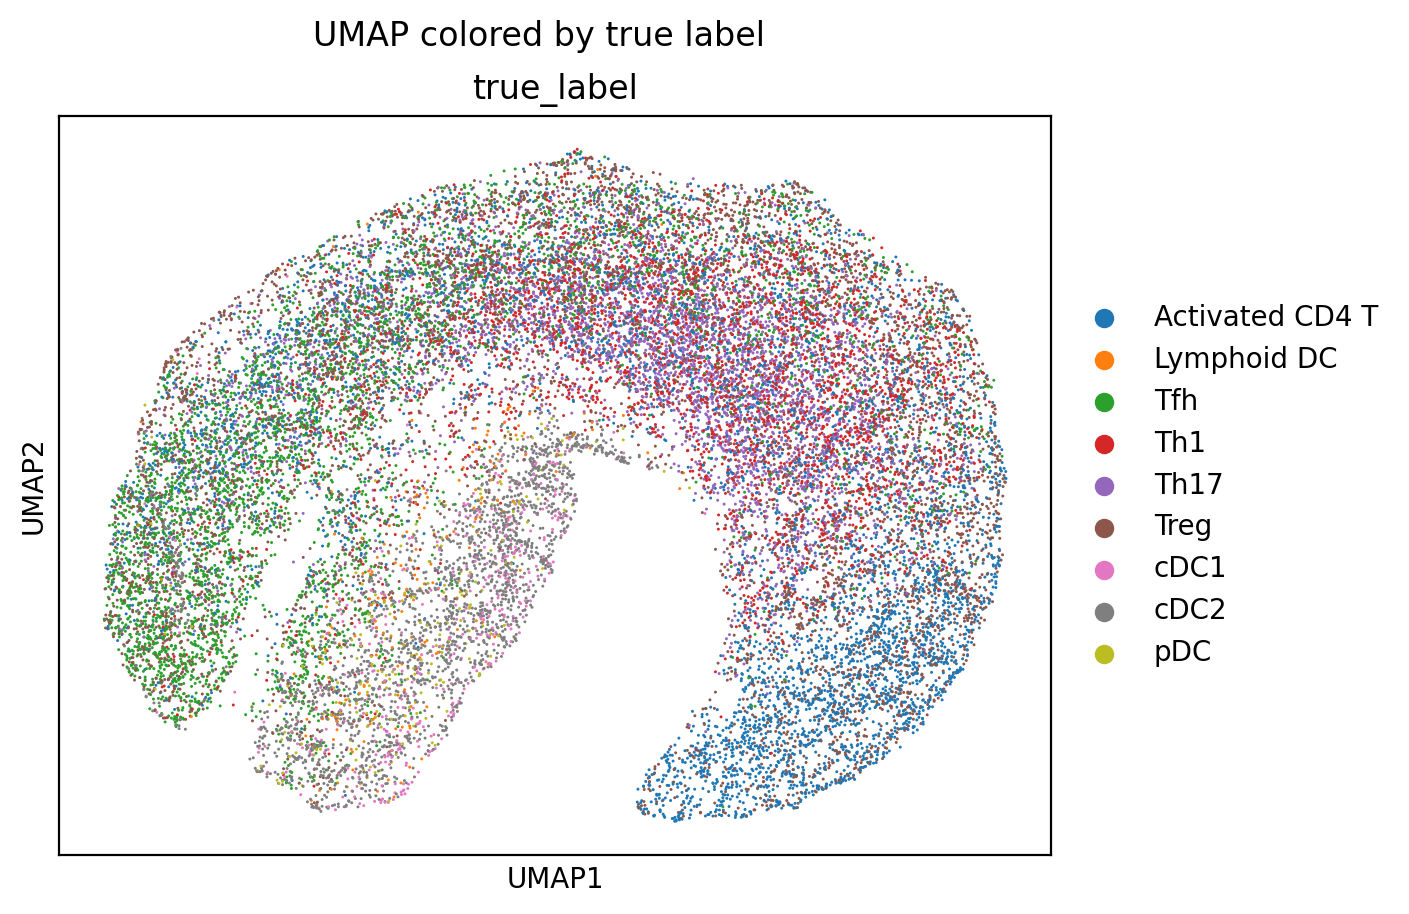
\includegraphics[width=\linewidth]{umap_true_label.png}
  \caption*{(a) UMAP colored by true label.}
\end{minipage}\hfill
\begin{minipage}{0.49\linewidth}
  \centering
  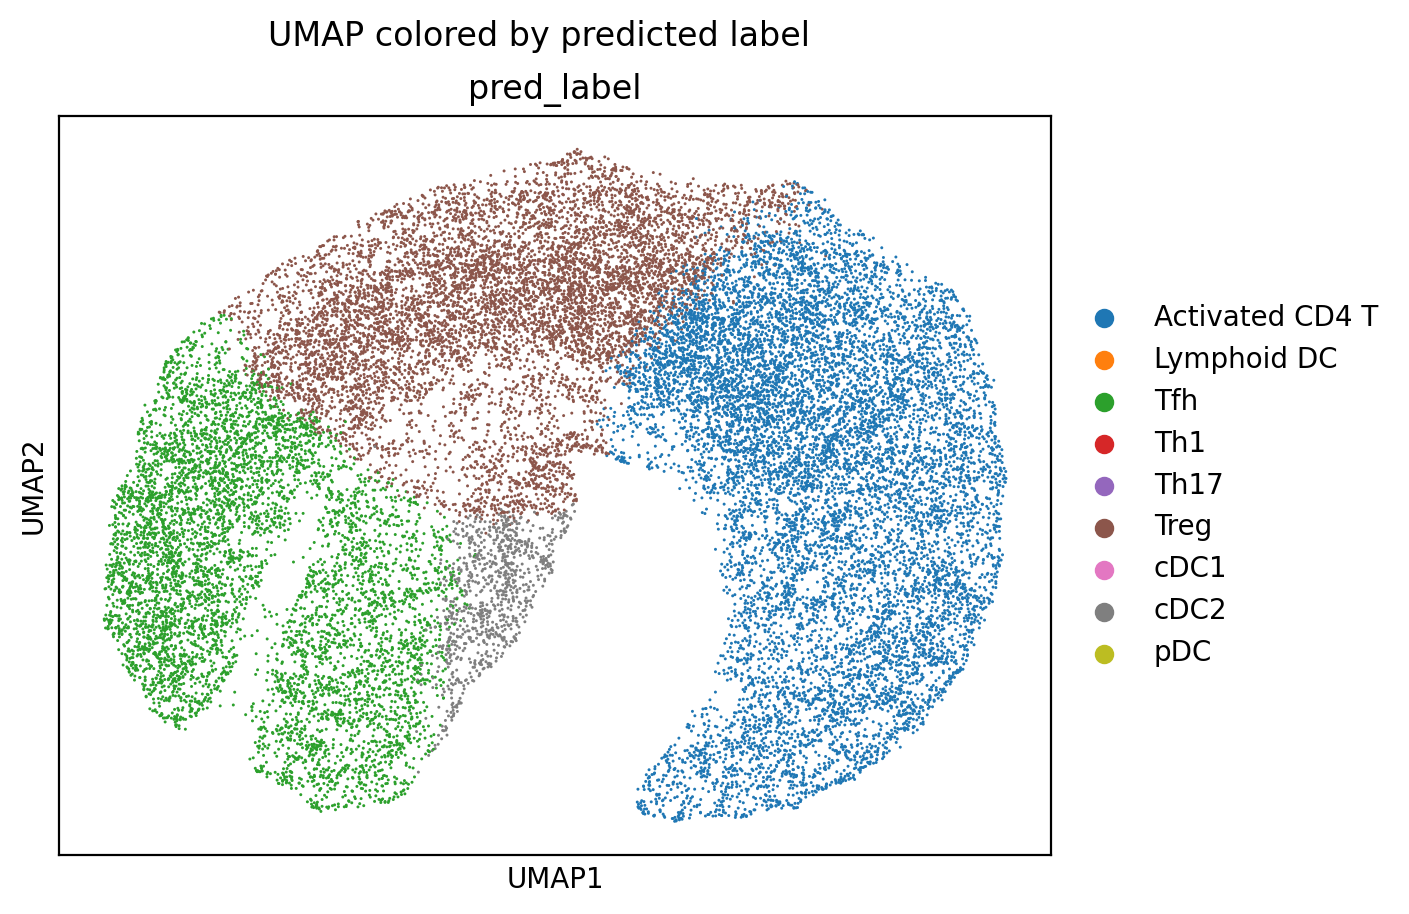
\includegraphics[width=\linewidth]{umap_pred_label.png}
  \caption*{(b) UMAP colored by predicted label.}
\end{minipage}
\caption{UMAP projections of the combined analysis set.}
\label{fig:umaps}
\end{figure}

\subsection{Baseline suite}
The repository already includes a benchmark baseline script so that future revisions can report the same task against simpler competitors.
The current suite covers majority-class prediction, PCA + logistic regression, PCA + linear SVM, PCA + kNN, and Leiden clustering.
Those methods are not yet expanded into a full results table in this initial manuscript, but they define the comparison frame for the next benchmark revision.

\begin{table}[H]
\centering
\caption{Planned baseline methods implemented in the repository benchmark suite.}
\begin{tabular}{ll}
\toprule
Family & Methods \\
\midrule
Simple classifier & Majority class \\
Linear probe & PCA + logistic regression \\
Linear probe & PCA + linear SVM \\
Instance-based & PCA + kNN \\
Graph clustering & Leiden \\
\bottomrule
\end{tabular}
\end{table}

\section{Discussion}
This run should be interpreted as a benchmark foundation, not as a final claim of biological or algorithmic superiority.
Its main value is that the complete experimental stack now works end to end: data preparation, model training, checkpoint recovery, evaluation, and figure generation.

The current performance is constrained by three obvious factors.
First, the transfer setting is strict: the model must cross atlas boundaries instead of solving a within-dataset split.
Second, the shared gene budget is small, with only 128 overlapping features after preprocessing.
Third, the reported result is a single-seed run, so we do not yet know the variance.

Those limitations are not flaws in the manuscript; they are the point of the benchmark.
A useful benchmark should make the hard part visible.
Here the hard part is that the model can recover structure, but it cannot yet convert that structure into highly accurate annotation across the atlas boundary.

\subsection{Auxiliary baseline calibration on PBMC68k\_reduced}
To verify the reporting stack and provide a concrete comparison table, we also ran the same baseline suite on \texttt{pbmc68k\_reduced}.
These results are calibration numbers rather than the main gut-atlas claim, but they let the manuscript report a complete baseline table in a publication-style format.

\begin{table}[H]
\centering
\caption{Auxiliary baseline calibration on PBMC68k\_reduced (seed 0).}
\label{tab:pbmc-baselines}
\begin{tabular}{lccccc}
\toprule
Method & Accuracy & Balanced acc. & Macro-F1 & ARI & NMI \\
\midrule
Majority class & 0.3429 & 0.1000 & 0.0511 & 0.0000 & 0.0000 \\
PCA + logistic regression & 0.7619 & 0.6597 & 0.6515 & 0.5788 & 0.7210 \\
PCA + linear SVM & 0.6857 & 0.6091 & 0.5805 & 0.5189 & 0.5818 \\
PCA + kNN & 0.7619 & 0.5602 & 0.5566 & 0.6144 & 0.6833 \\
Leiden clustering & 0.1238 & 0.2786 & 0.2184 & 0.5697 & 0.7121 \\
\bottomrule
\end{tabular}
\end{table}

\section{Limitations and Future Work}
The next revision of this benchmark should add several elements:
\begin{itemize}[leftmargin=1.2em]
  \item multiple random seeds with mean and standard deviation;
  \item the full gut-atlas baseline table with metrics for each method;
  \item ablation studies on gene selection and binning;
  \item a stronger transfer objective or regularization strategy;
  \item a clearer comparison to classical label-transfer systems.
\end{itemize}

A more complete paper version should also report training time, memory footprint, and sensitivity to shared-gene count.
Those numbers are especially relevant in a CPU-only setting, where usability matters as much as raw accuracy.

\section{Reproducibility}
The run is reproducible from the repository artifacts.
Key outputs are stored under the paper directory and the corresponding training run directory.
The main analysis artifacts are:
\begin{itemize}[leftmargin=1.2em]
  \item \texttt{summary.json}
  \item \texttt{final\_test.json}
  \item \texttt{analysis/metrics.json}
  \item \texttt{analysis/analysis\_input.h5ad}
  \item \texttt{analysis/umap\_true\_label.png}
  \item \texttt{analysis/umap\_pred\_label.png}
  \item \texttt{paper/baselines/pbmc68k\_seed0/summary.json}
\end{itemize}
Run directory:
\begin{quote}
\url{runs/annotation_smoke_retry2/gutatlas_transfer/scgpt/seed_0}
\end{quote}

For future benchmark revisions, the same protocol can be re-run with more seeds or alternative backbones while keeping the reporting structure unchanged.

\section{Conclusion}
We converted a fragile smoke test into a reproducible gut atlas transfer benchmark and documented the first complete end-to-end result.
The current scGPT configuration is stable and restartable, but its predictive quality is still too low for a strong benchmark claim.
That said, the experiment now has the structure of a real paper: a defined task, a clear protocol, explicit metrics, a reproducible artifact trail, and a natural path to stronger baselines.

\section*{Artifacts}
Run directory:
\begin{quote}
\url{runs/annotation_smoke_retry2/gutatlas_transfer/scgpt/seed_0}
\end{quote}

Metrics source files:
\begin{itemize}[leftmargin=1.2em]
  \item \texttt{summary.json}
  \item \texttt{final\_test.json}
  \item \texttt{analysis/metrics.json}
\end{itemize}

\begin{thebibliography}{9}
\bibitem{scgpt}
scGPT project.
\newblock \url{https://github.com/bowang-lab/scGPT}

\bibitem{celltypist}
CellTypist project.
\newblock \url{https://github.com/Teichlab/celltypist}

\bibitem{scanpy}
Scanpy project.
\newblock \url{https://scanpy.readthedocs.io/}
\end{thebibliography}

\appendix
\section{Implementation notes}
The repository contains a benchmark script that can be extended to produce the full comparison table.
The currently implemented baseline families are majority class, PCA + logistic regression, PCA + linear SVM, PCA + kNN, and Leiden clustering.
This appendix is intentionally practical: it records the baseline frame now, so that the next iteration only needs to fill in numbers.

\section{Known failure modes and mitigations}
Several small engineering issues were resolved while building the benchmark:
\begin{itemize}[leftmargin=1.2em]
  \item interrupted runs now resume from \texttt{last\_checkpoint.pt};
  \item bad cached downloads are detected and refreshed;
  \item singleton groups are filtered before marker analysis;
  \item analysis exports avoid mixed-type columns that break H5AD writing.
\end{itemize}

These fixes do not change the scientific claim, but they matter for repeatability.
A benchmark is only useful if it can survive ordinary execution failures.

\end{document}
